\debut{Emile Martinez}{Terminale (II) / MPI (III)}{Schéma entité association / Modèle relationnel}{}

Pendant toute la leçon on se base sur l'exemple suivant :

\begin{center}
	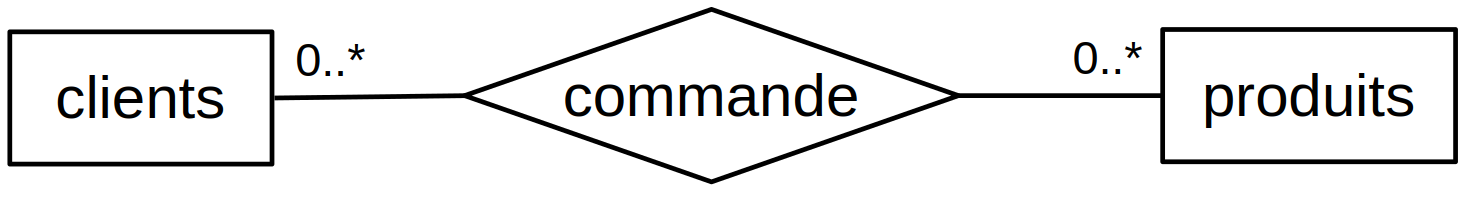
\includegraphics[width=0.6\linewidth]{lecon/28-sql/schema-EA.png}
\end{center}

\noindent \texttt{Produits(\underline{num\_produit}, nom, prix, poids)}\\
\texttt{Clients(\underline{num\_client}, nom, adresse, ville)}\\
\texttt{Commande(\underline{\#num\_produit, \#num\_client}, quantite)}

\section{Les tables}

\begin{definition}
	Une table est un tableau où chaque colonne est étiqueté par un attribut et contient des données du même type, et où chaque ligne est appelé un n-uplet, une entrée ou encore un enregistrement.	
\end{definition}

\begin{example}
	Table produits :
	\begin{center}
		\begin{tabular}{|c|c|c|c|}
			\hline num\_produit & nom & prix & poids \\ \hline
			1 & pomme & 1,5 & 1 \\ \hline
			2 & poulet & 7 & 2 \\ \hline
			3 & patate & 2 & 1 \\ \hline
		\end{tabular}
		\\
		\enspace \\
		\underline{produits}
	\end{center}
\end{example}

\section{Requêtes de bases (Terminale)}

\subsection{Requêtes de sélection}

Une requête de selection prend en entrée une ou plusieurs tables et les transforme en une nouvelle table.

\begin{syntaxe}
	\texttt{FROM} : appelle une table\\
	\texttt{SELECT} : selectionne les colonnes (projection)
\end{syntaxe}

\begin{example}
	Affichage du nom de tous les produits
	\begin{lstlisting}
SELECT nom
FROM produits
	\end{lstlisting}
\end{example}

\begin{syntaxe}
	\texttt{WHERE} est utilisé avant une sélection pour filtrer les n-uplets. Il est suivi d'une condition booléenne : seules les entrées la satisfaisant seront renvoyées
\end{syntaxe}

\begin{example}
	Affichage du nom des produits coutant moins que 50€
	\begin{lstlisting}
SELECT nom
FROM produits
WHERE prix < 50
	\end{lstlisting}
\end{example}

\begin{rem}
	Dans un \texttt{WHERE}, on a le droit aux opérations entières, à $<$, $>$, $=$, \texttt{AND}, \texttt{OR}, \texttt{NOT}
\end{rem}

\begin{syntaxe}
	\texttt{table1 \texttt{JOIN} table 2 \texttt{ON} condition} crée la table des éléments de table1 et de table2 (avec les colonnes des deux tables) en ne gardant que les lignes qui vérifient la condition.
	
	On peut alors renommer une table avec un alias après \texttt{AS} pour différencier les attributs de mêmes noms.
\end{syntaxe}

\begin{example}
	Les noms des produits présents dans une commande de gros (avec plus de 10 éléments)
	\begin{lstlisting}
SELECT p.nom
FROM produit AS p JOIN
     commande AS c ON p.num_produit = c.num_produit
WHERE c.quantite > 10
	\end{lstlisting}
\end{example}

\begin{syntaxe} Autres mot clefs :
	\begin{itemize}[label=]
		\item \texttt{DISTINCT} (après \texttt{SELECT}) pour ne garder que les lignes différentes
		
		\item \texttt{SELECT *} pour afficher toutes les colonnes
		
		\item \texttt{ORDER BY attributs ASC} (resp. \texttt{DESC}) (à la fin de la requête) qui trie les éléments par ordre croissant (resp. décroissant) selon attributs
		
		\item \texttt{LIMIT x OFFSET y} (à la fin de la requête) qui enlève les y premiers éléments et affiche seulement les x premiers restants
	\end{itemize}
\end{syntaxe}

\subsection{Invention et mise à jour}

\begin{syntaxe}[Requête d'insertion]
	On ajoute un n-uplet dans une table avec le mot-clef \texttt{INSERT INTO} suivi du nom de la table et du n-uplet.
\end{syntaxe}

\begin{example}
	\begin{lstlisting}
INSERT INTO produit VALUES (1, "baguette", 1.20, 200), 
                           (2, "pates", 1.5, 500)
;
	\end{lstlisting}
\end{example}

\begin{syntaxe}[Requête de suppression]
	 On utilise \texttt{UPDATE} et \texttt{SET} pour modifier les données d'une table, suivi d'un \texttt{WHERE} qui selectionne les lignes à modifier
\end{syntaxe}

\begin{example}
	\begin{lstlisting}
UPDATE produit SET prix = 1.3 WHERE id = 1;
	\end{lstlisting}
\end{example}

\begin{syntaxe}[Requête de supression]
	\texttt{DELETE FROM table WHERE condition} supprime de la table tous les n-uplets vérifiant cond
\end{syntaxe}

\begin{example}
	\begin{lstlisting}
DELETE FROM produit
WHERE id = 2
	\end{lstlisting}
\end{example}

\begin{proposition}
	Si une requête de modification viole une contrainte (clef primaire déjà présente, suppression d'un élément dont la clé est étrangère dans une autre table, etc.) la requête n'est pas effectuée
\end{proposition}

\paragraph{Développement : Premiers pas en SQL}

\section{Pour aller plus loin (Prépa)}

\subsection{Types de données en SQL}

SQL possède de nombreux types de données. Les types peuvent être numériques (\texttt{INT}, \texttt{DECIMAL}, \texttt{REAL}), textuels (\texttt{CHAR(n)}, \texttt{VARCHAR(n)}, \texttt{TEXT}) ou plus spécifiques comme \texttt{DATE} et \texttt{TIME}.\\

Sur ces types s'appliquent les opérations de comparaisons : \texttt{<=}, \texttt{<}, \texttt{=}, \texttt{<>} (= $\neq$),  \texttt{>}, \texttt{>=}

\begin{rem}
	Les types \texttt{DATE} et \texttt{TIME} sont des chaines de caractères. La comparaison se fait donc d'après l'ordre lexicographique. Néanmoins, leur format et tel que la comparaison est la même que selon la date représenté
\end{rem}

\begin{rem}
	Sur les types numériques il y a aussi les opérations mathématiques usuelles.
\end{rem}

\begin{definition}
	La valeur \texttt{NULL} représente l'absence de valeur
\end{definition}

\begin{proposition}
	Toute comparaison avec la valeur \texttt{NULL} donnera au final quelque chose de faux
\end{proposition}

\begin{example}
	\begin{lstlisting}
SELECT *
FROM produit
WHERE NOT(NULL = NULL) OR NOT(NULL <> NULL)
	\end{lstlisting}
renverra une table vide.
\end{example}

\begin{syntaxe}
	Pour tester si un attribut est à \texttt{NULL}, on utilise \texttt{IS NULL} et \texttt{IS NOT NULL}
\end{syntaxe}

\subsection{Requêtes ensemblistes}

Les opérateurs ensemblistes permettent de combiner dans un résultat unique des lignes provenant de deux (ou plus) requêtes. Les lignes peuvent venir de tables différentes mais après projection on doit obtenir des tables ayant même schéma de relation (même attributs).\\

Les opérateurs ensemblistes sont les suivants : 
\begin{itemize}[label=$\bullet$]
	\item \texttt{UNION} : pour obtenir l'union des deux requêtes

	\item \texttt{INTERSECT} : pour obtenir l'intersection des deux requêtes

	\item \texttt{EXCEPT} : pour obtenir la différence entre deux requêtes
\end{itemize}

\begin{example}
    Noms de tous les protagonistes de la base
	\begin{lstlisting}
SELECT nom FROM produit
UNION
SELECT nom FROM clients
	\end{lstlisting}
\end{example}

\begin{syntaxe}
	On peut également faire un produit cartésien de tables. On peut le faire avec un \texttt{JOIN . ON 1=1} mais on peut également simplement mettre une virgule entre tables \texttt{,} ce qui fera un produit cartésien.
\end{syntaxe}

\begin{exercise}
	Faire une jointure uniquement à l'aide de produit cartésien et de la clause \texttt{WHERE}
\end{exercise}

A mi-chemin entre le produit et la jointure il y a les jointures externes.

\begin{syntaxe}[Jointures externes]
	Dans une jointure externe, l'une des tables utilisées est directrice : tous ses renseignements seront présents dans la table résultante même s'ils n'ont pas de valeurs correspondantes avec les autres tables de la requête. Les colonnes de l'autre table seront alors remplies de \texttt{NULL}.
	\begin{itemize}
		\item \texttt{LEFT JOIN} : retourne tous les n-uplets de la table gauche même si la condition n'est pas vérifiée dans l'autre table
		\item \texttt{RIGHT JOIN} : retourne tous les n-uplets de la table droite même si la condition n'est pas vérifiée dans l'autre table
		\item \texttt{FULL JOIN} : union du left join et du right join
	\end{itemize}
\end{syntaxe}

\begin{com}
	Si on a la place ici on peut également mettre un exemple, e.g. (j'ai rien trouvé de super donc j'ai pas mis d'exemple, mais si on voulait afficher toutes les commandes mais que l'on voulait que tous les clients apparaissent)
\end{com}

\begin{syntaxe}
	On peut utiliser dans une clause de condition le mot clé \texttt{attributs IN requete} qui permet de savoir si attributs est présent dans le résultat de requête.
\end{syntaxe}

\begin{rem}
	On appelle cela une requête imbriquée.
\end{rem}

\begin{example}
	\begin{lstlisting}
SELECT VILLE
FROM CLIENTS
WHERE num_client IN (SELECT num_client FROM commandes)
	\end{lstlisting}
\end{example}

\subsection{Requêtes agrégatives}

\begin{definition}
	Un agrégat est un partitionnement horizontal d’une table en sous-table en fonction des valeurs d’un ou plusieurs attributs de partitionnement.
\end{definition}

\begin{personalise}[Schéma]
	\begin{tabular}{|c|c|}
		\hline 1 & pomme \\
		\hline 2 & poulet \\
		\hline 1 & navet \\
		\hline 2 & pomme \\
		\hline
	\end{tabular} $\qquad \to \qquad$ \begin{tabular}{|c|c|}
		\hline \multirow{2}{*}{1} & pomme \\
		\cline{2-2} & navet \\
		\hline \multirow{2}{*}{2} & poulet \\
		\cline{2-2} & pomme \\
		\hline 
\end{tabular}
\end{personalise}

\begin{syntaxe}
	\texttt{GROUP BY attribut} crée cette agrégation.
\end{syntaxe}

On peut alors appliquer des fonctions statistiques qui seront appliquées à chaque agrégat : \begin{itemize}[label=$\bullet$]
	\item \texttt{COUNT(*)} : compte le nombre de valeur de la sous-table
	\item \texttt{SUM(attribut)} : somme les valeurs de attribut sur la sous table
	\item \texttt{AVG(attribut)} : calcule la valeur moyenne
	\item \texttt{MAX} (resp. \texttt{MIN}) \texttt{(attribut)} : calcule la valeur maximum (resp. minimum)
\end{itemize}

\begin{syntaxe}
	Pour filtrer les sous-tables que l'on veut garder en utilisant après le \texttt{GROUP BY} par une clause \texttt{HAVING condition}, où la condition peut contenir des requêtes agrégatives.
\end{syntaxe}

\begin{example}
	Listes des villes ayant au moins 5 clients
	\begin{lstlisting}
SELECT ville
FROM clients
GROUP BY ville
HAVING COUNT(*) >= 5
	\end{lstlisting}
\end{example}

\paragraph{Développement 2 :} Requêtes avancées, avec ou sans agrégation